\begin{figure}[h!]
\centering
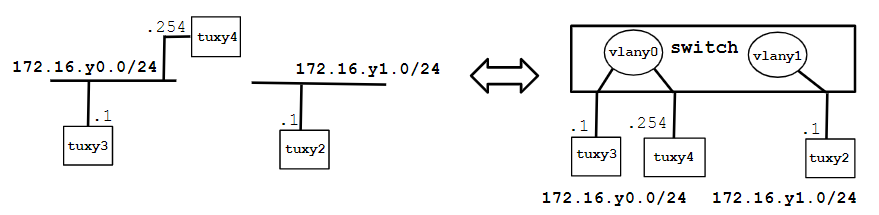
\includegraphics[scale=0.35]{imagens/Exp2.png}
\caption{Arquitetura da Segunda Experiência}
\label{fig:exp2}
\end{figure}

Esta experiência tem como objetivo a criação de duas VLAN's no switch e perceber a conectividade entre os tuxs, depois de os configurar em cada uma das sub-redes.

Os comandos usados para esta experiência podem ser encontrados no Anexo \ref{exp2_steps}.

\subsubsection{Análise dos Logs}

Para configurar as VLAN's criámos a VLAN 20 e 21 e associamos à primeira, os tux's 23 e 24 e à segunda o tux 22, com o objetivo de obter a arquitetura da figura 4.
Para testar a conectividade entre os tux's foi feito ping do tux23 até o tux24 que ocorreu com sucesso como seria de esperar uma vez que se encontram na mesma sub-rede, como se pode comprovar na Figura \ref{fig:exp2_tux23_ping_tux24}.

Quanto à conexão entre o tux23 e o tux22, o ping não obteve resposta devido ao facto de não haver nenhuma rota entre as VLAN's, sendo impossível o tux23 chegar à interface de rede do tux22.

Também no tux23 foi feito ping em broadcast, ping -b 172.16.20.255, que não obteve resposta, como demonstra o registo da Figura \ref{fig:exp2_tux23_broadcast}. Aqui, seria expectável uma resposta do tux24 uma vez que se encontram na mesma sub-rede, mas tal não acontece porque echo-ignore-broadcast está ativado por default para evitar grandes amplificações de tráfego. No entanto, os logs realizados no tux24 (Figura \ref{fig:exp2_tux24_broadcast}) comprovam que este recebeu um pedido do tux23 por broadcast.

Repetimos o processo anteriormente descrito mas agora a partir do tux22. Mais uma vez não obtivemos resposta, mas a justificação é diferente. Neste caso não foi obtida nenhuma resposta pois não está configurado mais nenhum dispositivo na VLAN 21 a não ser o próprio tux22. 

Assim, podemos concluir que exitem dois domínios de broadcast que correspondem às sub-redes VLAN 20 e VLAN 21 com os endereços 172.16.20.255 e 172.16.21.255, respetivamente.
